\documentclass[]{report}
\usepackage{graphicx}
\usepackage{todonotes}
\graphicspath{ {resources/images/} }


% Title Page
\title{Utilising peer-to-peer networking for data transfer over the browser}
\author{Dominic Rathbone}


\begin{document}
\maketitle
\tableofcontents
\listoftodos


\chapter{Interim planning \& investigation report}
	\section{Project Scope}
		\subsection*{Aims and Objectives}
			The ultimate objective of my project is to investigate the possibility of data transfer over web browsers (in particular audio and video streaming) without the need for a centralised client-server architecture, instead opting for a peer-to-peer network architecture. In order to do so, I will need to research peer-to-peer networking, multicasting as well as technologies that will allow for it's development in the browser such as WebRTC. On top of this, I will need to look into video streaming protocols and compression. In order to test and demonstrate this objective, It will materialize in the form of a web application that people can use to both transfer and stream files (if in a suitable format).
		\subsection*{Stakeholders}
			The stakeholders involved in my project will be myself, my supervisor, Stelios Kapetanakis and the user.
		\subsection*{Methods of communication}
			Stelios and I have set up a regular meeting once a week on Friday at 4pm to review progress and answer any questions. On top of this, we communicate regularly via email and I have set up a private git repository on GitHub to keep my project in which I will give Stelios access to. I have also got a kanban board set up on my 
			
	\section{Literature Review}
		\subsection*{Current solutions to data transfer}
			Currently, solutions such as DropBox and Google Drive mostly focus on cloud storage as a service whilst providing the ability to share the files they upload as a lesser function of their service. Whilst the files you upload can be encrypted in a way that means only clients of the service can decrypt them, many people feel insecure leaving traces of their private information on a remote server belonging to a company that has many interests it has to serve to. In 2013, this concern was legitimized by Edward Snowden when he disclosured information about government survelliance programs such as PRISM. PRISM coerced firms such as Google, Microsoft and Yahoo to provide private data from citizens using their services to the government. \cite{PRISM}  More recently, this idea has been reinforced by legislation such as the "Investigatory Powers Bill"  being introduced in the UK that prohibits internet companies to offer encryption that they cannot break in order to allow the government to collect decrypted data from them. 
			
			As an alternative to using cloud storage solutions for sharing files, there is also specific file sharing sites such as WeTransfer that allows you to send files up to 2gb via their site. This works by sending a link through email to the person you want to send the file to. Whilst it does store the uploaded files, they are only kept for 7 days in order to prevent unnecessary storage usage \cite{WeTransfer Storage Time}. Although this is better for data privacy, WeTransfer use third party providers such as Amazon Web Services (AWS) to store this data (using AWS S3 Storage) \cite{WeTransfer AWS Case Study} meaning there is still the potential concern of data privacy highlighted previously.
			
			There are also further alternatives to the traditional client-server file transfer architectures such as sharefest.me
			\todo{Current peer to peer solutions}
			
		\subsection*{Comparing network architectures}
			The most common architecture for these file storage/transfer and video streaming services is the client-server model. This is an network architecture in which the machines doing the data processing (servers) are separated from the machines running the application (client). Whilst the shift of processing on to the service supplier means that the user of the application does not need a powerful machine to run it, it also means that the service supplier has the responsibility of maintaining and paying for these servers. Furthermore, although modern server architectures are designed in a distributed structure granting them to be more robust, if these servers becomes congested as load increases or in extreme cases, if the servers go down, the user would not be able to use the application as intended. Using a decentralized peer-to-peer networking architecture avoids both these issues as processing is distributed between the peers making up the network, resulting in it being cheaper to maintain and scale the service as load increases whilst being inherently robust. However, there are a number of considerations to regard in peer to peer networking.
		
			Security is a concern within peer-to-peer networking as there is no centralized authority to manage access control to resources. Thus in a decentralised network, a malicious client could potentially launch a number of attacks versus other nodes in the network such as Denial Of Service (DoS) where a malicious group of nodes floods a network with a massive amount of fake data, potentially crashing nodes within it or Man in the Middle (MitM) attacks where a node is able to intercept data flowing between two other nodes and spy on or poison this data.\cite{P2P Security Issues}
			
			Whilst it would be hard to completely avoid risks like this as it is an inherent flaw in peer-to-peer architecture, introducing the basic concept of trust into a peer-to-peer network can stop malicious peers from entering it in the first place. I could implement this by allowing users of the application to enable authentication on the page where the connection lies would give them a level of access control that would stop malicious peers that would be able to join. Note as well, the technology I am using to implement the peer-to-peer network, WebRTC, does seem to take this issue of security into account and secures the connection between two peers through a protocol called Datagram Transport Layer Security and Secure Real Time Protocol (DTLS-SRTP)\cite{WebRTC Security Study}.
	
		
		\subsection*{Peer-to-peer networking topology}
			The entire idea behind my application is based on this peer-to-peer connection between two browsers. Whilst this one-to-one (unicast) connection is formed and maintained by WebRTC, it does no more than this. To form a many-to-many (multicast) network, I will have to organise this at the application layer.
		
			A network can be structured in different ways, this structure is referred to as it's topology. There are several different network topologies but I plan to focus on mesh networking as I feel it would best represent the structure that the network of peers using my web application would form. 
			\todo{Network topology}
		
		\subsection*{WebRTC}
			WebRTC is an emerging web technology that enables browsers to communicate real time via a peer-to-peer connection, avoiding the need for a centralized server to transfer data between them. This was first released by Google as an open source project to implement real-time communication in the browser in May 2011 \cite{Google WebRTC Release}. It was later drafted as an API definition by W3C which is still a work in progress. \cite{W3C WebRTC Definition}. WebRTC has yet to be fully implemented in every web browser but Chrome, Firefox and a WebRTC specific browser called Bowser are leading the way in implementing the API definition. Firefox (Nightly) seems to be leading the way in this so I will focus specifically in developing towards this browser\cite{WebRTC browser support}.
			The 3 main WebRTC APIs supported at this time are:
				\begin{itemize}
					\item RTCDataChannel:
					"The RTCDataChannel interface represents a bi-directional data channel between two peers of a connection." \cite{Mozilla Web API} \todo{reword}
					\item RTCPeerConnection:
					"The RTCPeerConnection interface represents a WebRTC connection between the local computer and a remote peer. It is used to handle efficient streaming of data between the two peers." 
					\cite{Mozilla Web API} \todo{reword}
					\item getUserMedia:
					"Prompts the user for permission to use one video and/or one audio input device such as a camera or screensharing and/or a microphone. If the user provides permission, then the successCallback is invoked with the resulting MediaStream object as its argument. If the user denies permission or media is not available, then the errorCallback is called with PermissionDeniedError or NotFoundError respectively. Note that it is possible for neither completion callback to be called, as the user is not required to make a choice."
					\cite{Mozilla Web API} \todo{reword}
				\end{itemize}
			My Web Application will utilize the RTCPeerConnection and RTCDataChannel APIs. The former to establish a peer connection between two clients and the latter to create a data channel over this peer connection to transfer data.
			
			Although WebRTC is used to transfer data, it purposely doesn't handle signalling. Signalling is a concept that came from telecommunications and VoIP. It is the process of organising the communication between two clients and handles the exchange of metadata that creates and manages a session between two clients. With WebRTC, the most prevalent signalling protocol is the Session Initiation Protocol (SIP). SIP 
			\todo{SIP}
				
			This data is sent over a protocol called Secure Real Time Transport Protocol (SRTP). This protocol was originally developed for secure VoIP but has been adopted by WebRTC. 
			\todo{DTLS - SRTP}	
		
		\subsection*{Media streaming}
			\todo{Media Streaming}
		\subsection*{BackBoneJS framework}
			\todo{JavaScript Framework}
			
	\section{Specification}
			\subsection*{Deliverables}
			The first intermediate product will be the signalling server written in Java. This will handle the exchange of client meta data in order to establish the connection between two peers using the web application. I plan to overlap the development of this with the development of the data transfer functionality and user interface of my second deliverable, the web application as manually testing the signalling server will be a lot easier with a partially developed application to test it with.
			
			The first end deliverable will be the client side web application the user interacts with in order to select a file as 	well as handling sending the meta data to the signalling server and managing the peer-to-peer data transfer and media streaming. This is broken down into several intermediate products, the data transfer functionality, the media streaming functionality, the many-to-many networking functionality and the user interface. I plan to produce the data transfer functionality first along side the user interface to allow for manual testing. After I have implemented data transfer, I will work on media streaming and forming the peer-to-peer network topology. 
			
			The second end deliverable will be the final report containing documentation and analysis using the metrics	from my application, comparing how it and technologies behind it perform in comparison to others, focusing in particular on how peer-to-peer over the browser (WebRTC) compares to other methods of data transfer and media streaming.
			\todo{schedule of activities}
			
			\subsection*{Risk analysis}
			\todo{risk table}
			In terms of risk, I think this will be the largest in my project as it is the only tangible end product and it relies on WebRTC which is a relatively immature technology. As it is new (released in 2011) and it is the only technology at the moment enabling browsers to communicate peer-to-peer, it has not truly been tried and tested. This means there is a higher potential for problems such as security flaws to exist. 
		
			\subsection*{Quality Analysis}
			Success will be measured by the performance of the web application's ability to transfer data. This will be achieved by application metrics recording how fast/reliably files are transferred under differing amounts of load. Load will be simulated using a load testing tool to mock client connections to the web application. I will implement metrics using the WebRTC statistics API, which allows for monitoring of peer connections.
			\todo{write more}
		
			
			
	\section{Methodology}
		I chose to use an alternative methodology to the waterfall model because the waterfall model lacks the ability to adapt to changes in a project deadline. Due to the way waterfall is structured into different phases that must be completed sequentially, often when changes such as new requirements occur, all these phases must be repeated in order to account for this. Iterative methodologies take an approach that can adapt to these changing requirements because they utilise short development cycles and focus on developing small modules of a product at one time, making it easier to revise a product if necessary. This is particular useful in my project as it is relatively experimental and the requirements of it may change regularly. 
		
		Thus, as a way of tracking the progression of my project, I plan to use Kanban methodology. This is used within software development as a way of incrementally developing applications through iterative cycles. Whilst it is similar to scrum, it does not have the stricter framework surrounding it that requires a product owner and scrum master. It also avoids overloading developers with restrictive time-boxed sprints. This methodology is relatively simple and is based around a backlog of tasks from which a developer pulls from in a limited amount, normally 1 or 2 tasks at a time which will are then pushed through the development work flow.
		
		In my case, the work flow will be relatively simple:
		\begin{enumerate}
			\item To Do
			\item In Progress
			\item Code Review
			\item Manual Testing
			\item Done
		\end{enumerate}
		During the "In Progress" step of the work flow, I will use a test driven development (TDD) process in which tests are written first and then code is wrote to make the test work. However, I will be fairly lenient with this, only using this process on parts of the code that require stringent testing as writing unnecessary tests will take up development time. 
		
		\begin{center}
			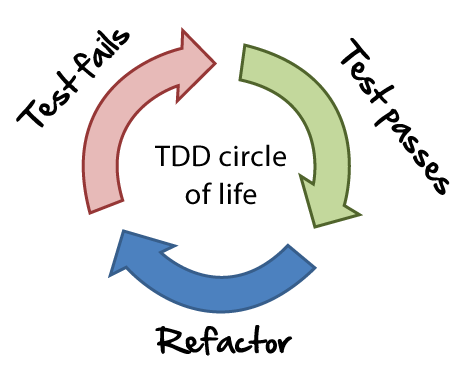
\includegraphics[scale=0.5]{tdd-circle-of-life.png}
		\end{center}
		
		During the "Code Review" step, I plan to self-evaluate the task I have completed. On top of this, I will run static code analysis tools (such as FindBugs and PMD for Java) if the task is a coding task and use the code review section StackExchange to get second opinions. If it passes the code review step and it is possible to do so, I will black-box test the task from a user's perspective to see that it actually works as intended. Once every task forming a feature is completed, I will manually test the feature as a whole to see that each task has integrated together as planned.
		
		\subsubsection*{Tools and Environment}
		\todo{Tools and environment}
		Git
		IDE
		Unit testing framework
		build tools
		
	\begin{thebibliography}{9}
		\bibitem{PRISM}
		Greenwald, Glenn; MacAskill, Ewen (June 6, 2013). "NSA Taps in to Internet Giants' Systems to Mine User Data". The Guardian.  Last accessed 05/11/2015.
		\bibitem{WeTransfer Storage Time}
		WeTransfer. How long are my uploads available to download?. Available: https://wetransfer.zendesk.com/hc/en-us/articles/202603916-How-long-are-my-uploads-available-to-download-. Last accessed 05/11/2015.
		\bibitem{WeTransfer AWS Case Study}
		Amazon Web Services. WeTransfer Case Study. Available: https://aws.amazon.com/solutions/case-studies/wetransfer/. Last accessed 05/11/2015.
		\bibitem{P2P Security Issues}
		Schulzrinne, et al.. (February 2010). Security in P2P Realtime Communications. Available: https://tools.ietf.org/html/rfc5765#section-7.2. Last accessed 05/11/2015.
		\bibitem{WebRTC Security Study}
		N/A. A Study of WebRTC Security. Available: http://webrtc-security.github.io/#4.3. Last accessed 05/11/2015.
		\bibitem{Google WebRTC Release}
		Harald Alvestrand. (2011). Google release of WebRTC source code. Available: http://lists.w3.org/Archives/Public/public-webrtc/2011May/0022.html. Last accessed 29/10/2015.
		\bibitem{W3C WebRTC Definition} 
		Adam Bergkvist, Daniel C. Burnett, Cullen Jennings, Anant Narayanan (until November 2012). (2011). WebRTC 1.0: Real-time Communication Between Browsers. Available: http://www.w3.org/TR/webrtc/. Last accessed 29/10/2015.
		\bibitem{WebRTC browser support}
		Available: http://iswebrtcreadyyet.com/. Last accessed 30/10/2015.
		\bibitem{Mozilla Web API}
		Mozilla Web API. Available: https://developer.mozilla.org/en-US/docs/Web/API. Last accessed 30/10/2015.
		\bibitem{Mesh Network Definition}
	\end{thebibliography}

\end{document}          
